For both versions of the robot, the transformation matrix values were determined using Denavit–Hartenberg (DH) parameters. When solving the kinematics for both v1 and v2, the length of the common normal was identified by the variable r to avoid confusion between variables a and $\alpha$. 

\subsection{Robot Configuration Overviews}
AFER v1 was a 2-DOF robot, actuated by servomotors and an Arduino controller, and modeled such that the cat toy end effector formed a rigid linkage with \textit{l2}. The robot utilized a revolute base joint (J1) and a revolute lift joint (J2) to move the end effector as commanded; the chosen joint configuration allowed the robot to operate along the edges of a hemispherical work envelope with a surface area of $39.9ft^2$, situated about the robot’s center, shown in Fig.5.

\begin{figure}[h!]
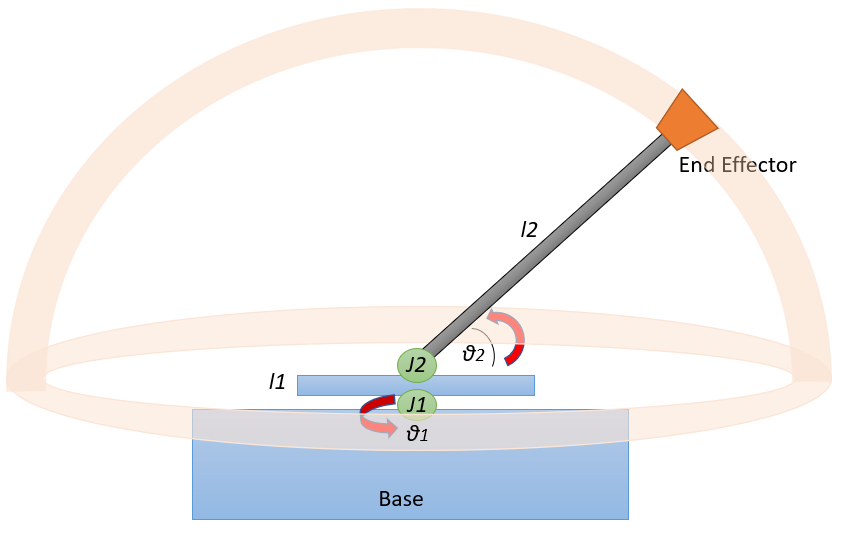
\includegraphics[width=\columnwidth]{Fig5.png}
\caption{AFER v1 Work Envelope.}
\label{fig5}
\end{figure}

For this version of the robot, the end effector was mounted directly to \textit{l2}. As the arrangement caused no considerable difficulty when solving the kinematic equations, the mathematical modeling used for v1 closely resembled the real-world robotic build, and the assumptions when solving the kinematic equations were minimal. 
For AFER v2 as shown in Fig.6, the cat toy end effector attached to the rest of the robot via J3, a frictionless joint that was passive in the pitch direction and had no damping. The chosen joint configuration allowed the robot to operate along the edges of a hemispherical workspace with a surface area of $39.9 ft^2$, situated about the robot’s center. The workspace size of v1 and v2 were identical, however the v2 workspace was lower due to the introduction of \textit{l3}. 


\begin{figure}[h!]
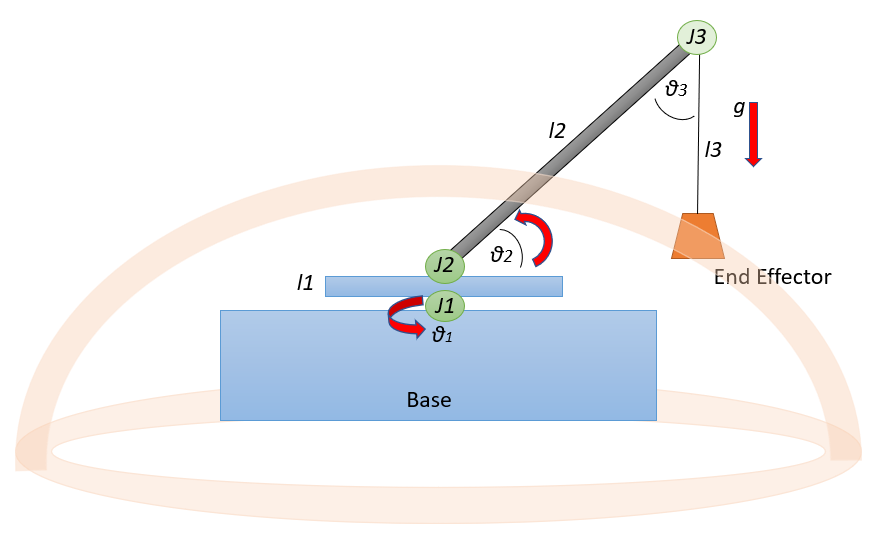
\includegraphics[width=\columnwidth]{Fig6.png}
\caption{AFER v2 Work Envelope.}
\label{fig6}
\end{figure}

Realistically, the string attached to the J3 joint on AFER v2 was able to move freely and had factors such as elasticity and conflicting multi-modal vibrations. However, it caused the kinematic equations to be non-linear and extremely difficult, if not impossible, to solve. Therefore, in order to ensure that the kinematics for this version of the robot were useful and solvable, J3 was modeled as a passive joint on a rigid link instead of a compliant linkage. Additionally, the momentum was discounted and the gravity(g) was assumed to be the only force acting upon the suspended end effector. 

\subsection{AFER v1 Forward Kinematics}
The forward kinematics for v1 as a 2-joint robot were relatively simple, but to ensure the solvability of the kinematic model, static stability was assumed for all points. Using the coordinate frames as shown in Fig.5, creating a transformation matrix from the base of the robot to the end effector using a link coordinate diagram was straightforward. The transformation values of r, $\alpha$, d, and $\theta$ are given in Table ~\ref{table:1}.

\begin{center}
\begin{table}[h!]
\centering
\caption{DH PARAMETERS FOR AFER v1}
   \begin{tabular}{ | c | c | c | c | c | }
   \hline
    Point & $d_{i}$ & $\theta_{DHi}$ & $r_{i}$ & $\alpha_{i}$ \\ \hline
    J1 & 0 & 0 & 0 & 0  \\ \hline
    J2 & \textit{l1} & $\theta_{1}$ & 0 & 0 \\ \hline
    EE & \textit{l2} & 0 & 0 & $\theta_{2}$\\ \hline
    \end{tabular}
		\label{table:1}
\end{table}
\end{center}

AFER v1 had a horizontal stroke equal to the length of \textit{l2} and a vertical stroke of \textit{l1} + \textit{l2}. Additionally, the absence of linear actuators indicated that the di values were static. The transformation from the coordinate frame at J1 to the coordinate frame at the end effector was determined as shown in \eqref{1}:

\[
\centering
\begin{bmatrix}
cos\theta_{1} & -sin\theta_{1}cos\theta_{2} & sin\theta_{1}sin\theta_{2} & 0\\
sin\theta_{1} & cos\theta_{1}cos\theta_{2} & -cos\theta_{1}sin\theta_{2} & 0 \\
0 & sin\theta_{2} & cos\theta_{2} & \textit{l2} + \textit{l1} \\
0 & 0 & 0 & 1 \\
\end{bmatrix}
\begin{equation}
\label{eq1}
\end{equation}
\]


\subsection{AFER v2 Forward Kinematics}
The forward kinematics for AFER v2, a 3-joint robot, were relatively simple. When solving the kinematics, static stability was assumed. The DH parameters for J1, J2, and J3 in v2 were identical to the DH parameters for J1, J2 and the end effector (E) of v1 due to the common core configuration of the robot. The values for v2 DH parameters are listed below in Table ~\ref{table:2}. 

\begin{center}
\begin{table}[h]
\centering
\caption{DH PARAMETERS FOR AFER v2}
    \begin{tabular}{ | c | c | c | c |c | }
    \hline
    Point & \ $d_{i}$ & $\theta_{DHi}$ & $r_{i}$ & $\alpha_{i}$ \\ \hline
    J1 & 0 & 0 & 0 & 0  \\ \hline
    J2 & \textit{l1} & $\theta_{1}$ & 0 & 0 \\ \hline
    J3 & \textit{l2} & 0 & 0 & $\theta_{2}$\\ \hline
		E & -\textit{l3} & 0 & 0 & $\theta_{2}+ \frac{\pi}{2}$ \\ \hline
    \end{tabular}
		\label{table:2}
\end{table}
\end{center}

As in v1, v2 had a horizontal stroke equal to the length of \textit{l2}; however, the vertical stroke of \textit{v2} was equal $\textit{l1} + \textit{l2} – \textit{l3}$. Given that there were no linear actuators, the $\textit{d}_{i}$ values were static. The transformation from the coordinate frame at J1 to the coordinate frame at the end effector(E) for v2 was determined as shown in \eqref{2}, where $(\alpha_{E} = \theta_{2} + \frac{\pi}{2})$.

\[
{\tiny
\centering
\label{eq2}
\begin{bmatrix}
c\theta_{1} & -s\theta_{1}c\theta_{2}c\alpha_{E} + s\theta_{1}s\theta_{2}s\alpha_{E} & s\theta_{1}c\theta_{2}s\alpha_{E} + s\theta_{1}s\theta_{2}c\alpha_{E}& -\textit{l3}s\theta_{1}s\theta{2}\\
s\theta_{1} & c\theta_{1}c\theta_{2}c\alpha_{E} - c\theta_{1}s\theta_{2}s\alpha_{E}  & c\theta_{1}c\theta_{2}s\alpha_{E} - c\theta_{1}s\theta_{2}c\alpha_{E}  & 0 \\
0 & s\theta_{2}c\alpha_{E}+ c\theta_{2}s\alpha_{E} & -s\theta_{2}c\alpha_{E}+ c\theta_{2}s\alpha_{E} & -c\theta_{2}\textit{l3} + \textit{l2} +\textit{l1} \\
0 & 0 & 0 & 1 \\
\end{bmatrix}
}
\begin{equation}
\label{eq1}
\end{equation}
\]

\subsection {AFER v1 Inverse Kinematics}
Based upon the hemispherical geometry and low degrees of freedom present in v1, it was simple to solve for the joint angles based on the position of the end effector. Basic trigonometric functions were leveraged to solve for $\theta_{2}$. Since the high torque servomotor creating $\theta_{2}$ had a maximum range of $180^{\circ}$, there was only one solution as in (3).

\begin{equation}
\theta_{2} = sin^{-1}\frac{E_{z} - \textit{l1}}{\textit{l2}} \label{eq3}
\end{equation}

It was easiest to solve for the rotational joint at $\theta_{1}$ by projecting J1 into the $x_{1}, y_{1}$ plane. This allowed the rotational displacement of the joint to be calculated using the simple trigonometric relationships. Due to ambiguity when solving with inverse cosine, inverse tangent was selected for solving for $\theta_{1}$. Since the servomotor at J1 could rotate a full $360^{\circ}$, there were two possible solutions for this joint angle, as (4) and (5) show.


\begin{equation}
\theta_{1} = tan^{-1} 2(E_{x},E_{y})\label{eq4}
\end{equation}

\begin{equation}
\theta_{1} = \pi + tan^{-1} 2(E_{x},E_{y})\label{eq5}
\end{equation}

\subsection{AFER v2 Inverse Kinematics}
For $\theta_{1}$ and $\theta_{2}$, the v2 inverse kinematics was identical to the v1. Solving for $\theta_{3}$ was trivial using the mathematical properties of triangles. Given that the sum of the interior angles of a triangle are always equal to $180^{\circ}$, and the assumption of static stability for J3, (6) was used to define $\theta_{3}$:

\begin{equation}
\theta_{3} = \frac{pi}{2} - \theta_{2} \label{eq6}
\end{equation}

